\documentclass[9pt,twocolumn,twoside,lineno]{pnas-new}
% Use the lineno option to display guide line numbers if required.

\usepackage{siunitx}
\usepackage{multirow}
\usepackage{color,soul}
\usepackage{xspace}
\usepackage{xcolor}

\newcommand{\red}[1]{\textcolor{red}{#1}}
\newcommand{\blue}[1]{\textcolor{blue}{#1}}

\templatetype{pnasresearcharticle} % Choose template 
% {pnasresearcharticle} = Template for a two-column research article
% {pnasmathematics} %= Template for a one-column mathematics article
% {pnasinvited} %= Template for a PNAS invited submission

\title{Modeling the Liquid-Liquid Phase Transition Induced by Polymerization}

% Use letters for affiliations, numbers to show equal authorship (if applicable) and to indicate the corresponding author
\author[a]{Nikolay A. Shumovskyi}
\author[b]{Thomas J. Longo} 
\author[a,c,1]{Sergey V. Buldyrev}
\author[b,d]{Mikhail A. Anisimov}

\affil[a]{Department of Physics, Boston University, Boston, MA 02215, USA}
\affil[b]{Institute for Physical Sciences and Technology, University of Maryland at College Park, MD 20742, USA}
\affil[c]{Department of Physics, Yeshiva University, New York, NY 10033, USA}
\affil[d]{Department of Chemical and Biochemical Engineering, University of Maryland at College Park, MD 20742, USA}

% Please give the surname of the lead author for the running footer
\leadauthor{Shumovskyi} 

% Please add a significance statement to explain the relevance of your work
\significancestatement{Our study provides a novel approach to understanding the phenomenon of liquid-liquid separation induced by polymerization, dimerization, or gelation in systems exhibiting polyamorphism (the existence of multiple amorphous states in a single component substance), such as hydrogen, sulfur, phosphorous, liquid carbon, selenium, tellurium, and biopolymers. Our results show that the developed model qualitatively reproduces the liquid-liquid phase transition in polymeric sulfur at high pressures and temperatures, which was recently experimentally observed in liquid sulfur.}

% Please include corresponding author, author contribution and author declaration information
\authorcontributions{The model was conceived by Sergey V. Buldyrev, then all the authors equally contributed to this study.}
\authordeclaration{The authors declare no competing interests.}
\correspondingauthor{\textsuperscript{1}To whom correspondence should be addressed. E-mail: buldyrev@yu.edu}

% At least three keywords are required at submission. Please provide three to five keywords, separated by the pipe symbol.
\keywords{Phase Separation $|$ Polymerization $|$ Sulfur $|$ Molecular Dynamics $|$ Liquid Polyamorphism} 

\begin{abstract}
We suggest a simple model to describe phase separation induced by polymerization, as was recently observed in liquid sulfur (\textit{Nature}, \textbf{584}, 382, 2020). The model contains three types of interactions: i) atoms attract each other by van der Waals forces which produce the liquid-gas phase transition at low pressures, ii) atoms may form covalent bonds which induce polymerization, and iii) polymerized atoms attract each other by van der Waals forces stronger than nonpolymerized atoms. We show that the latter interaction couples polymerization with phase segregation and produces the liquid-liquid phase transition that was recently observed in sulfur. We implement these three conditions using a discrete molecular dynamics approach. The phase diagram and structure factor demonstrate a qualitative agreement with the behavior of real sulfur.
\end{abstract}

\dates{This manuscript was compiled on \today}
\doi{\url{www.pnas.org/cgi/doi/10.1073/pnas.XXXXXXXXXX}}

\begin{document}

\maketitle
\thispagestyle{firststyle}
\ifthenelse{\boolean{shortarticle}}{\ifthenelse{\boolean{singlecolumn}}{\abscontentformatted}{\abscontent}}{}

% If your first paragraph (i.e. with the \dropcap) contains a list environment (quote, quotation, theorem, definition, enumerate, itemize...), the line after the list may have some extra indentation. If this is the case, add \parshape=0 to the end of the list environment.
\dropcap{A}bove $\SI{160}{\degreeCelsius}$, at ambient pressure, sulfur polymerizes with a sharp increase in viscosity, which has been interpreted as a ``lambda transition'' to a polymerized state \cite{Sauer_Lambda_1967,Bellissent_Sulfur_1994,Kozhevnikov_Sulfur_2004}. However, with further increase of temperature, as the system approaches the liquid-gas phase transition (LGPT), the polymer chains gradually dissociate and the viscosity decreases. Previous studies of sulfur have predicted a liquid-liquid phase transition (LLPT) at very high pressures, based on its electronic properties \cite{Brazhkin_PT_1999}. Contrarily, more recent \textit{ab initio} molecular dynamics simulations predicted a continuously decreasing average polymer chain length upon heating at $\SI{10}{\giga\pascal}$, not associated with a change in density \cite{Plasienka_Structural_2015}. Recently, it was discovered that high-density sulfur, well above the liquid-gas critical pressure (in the range from $0.5$ to $\SI{2.0}{\giga\pascal}$), exhibits a LLPT indicated by a discontinuity in density from a low-density liquid (LDL) to a high-density liquid (HDL) \cite{Henry2020}. This LLPT in polymerizing substances has also been observed in phosphorous \cite{Katayama2000} and liquid carbon \cite{Glosli_Liquid_1999}, while being proposed to exist in selenium and tellurium \cite{Brazhkin_PT_1999,Plasienka_Structural_2015}. 

The coexistence of two alternative liquid phases in a single component substance, like sulfur, is known as ``liquid polyamorphism'' \cite{Anisimov2018,Tanaka_Liquid_2020}, which was first observed by molecular dynamics simulations of classical all-atom models of supercooled water \cite{Poole1992,Debenedetti2020,Speedy1976,Gallo2016}. This phenomenon can be understood via two-state thermodynamics \cite{Holten2001,Caupin2021}, in which two alternative molecular or supramolecular states may interconvert via a reversible reaction \cite{Longo2021,Caupin2021}. In spite of the significant recent progress \cite{Kim2020}, no definitive experimental confirmation of a liquid-liquid transition in water has been found yet \cite{Tanaka_Liquid_2020}. 

%
%Liquid polyamorphism is proposed to be the cause of the anomalies observed in deeply supercooled water.

Computationally, a LLPT has also been observed in single-component systems with core soften potentials \cite{Stell1972,Stillinger1993,Jagla2001,Franzese2001,Gibson2006,Skibinsky2004}, \emph{e.g.} a spherically symmetric potential consisting of a wide attractive well and a repulsive shoulder. In such models, the particles may acquire alternative local structures, forming high-density and low-density phases, which can be understood through the two-state idea. In this work, using this approach, we propose a maximum-valence model \cite{Zaccarelli2005,Debenedetti,Debenedetti2} where atoms may form covalent bonds via a reversible reaction, changing their state according to the number of bonds they have with other atoms. We assume that the atoms form linear polymers with a maximum of two bonds per atom, mimicking the valence structure and bond formation similar to sulfur. We consider the scenario where polymerized atoms (with two bonds) attract each other stronger than the other unbonded atoms and single-bonded atoms in the system. Our molecular dynamics (MD) simulations demonstrate that this model is able to qualitatively reproduce the LLPT observed in sulfur, and demonstrates that the polymerization reaction is the cause of this liquid-liquid phase separation.

\section*{Maximum-Valence Model}
We model the polymerization of a sulfur-like system by characterizing each atom by its coordination number, the number of bonds it has with other atoms. Depending on the coordination number, each atom is assigned to distinguished states: S$_0$ (with zero bonds), S$_1$ (with one bond), and S$_2$ (with two bonds). Atoms cannot form more than two bonds and, consequently, will polymerize into a linear polymer. All of the atoms in the system may change their state by forming or breaking a covalent bond via a reversible reaction. Fig.~\ref{fig1}a depicts the three types of reversible reactions that may occur in the system. In this work, we demonstrate that the minimum ingredients required to produce a LLPT are the following: i) the van der Waals interactions between atoms, which produce a LGPT; ii) covalent bonds between atoms, which induce polymerization; and iii), as we hypothesize, additional van der Waals interactions between atoms with maximum valency (having two bonds), which couple phase segregation to polymerization. These three ingredients are illustrated by square-well potentials in Figs.~\ref{fig1}(b-d). \red{Physically, the additional attraction between atoms in neighboring chains may stem from the fact that in real polymers the covalent bond is shorter than the diameter of the unbonded (``free'') atoms, such that the attractive wells of bonded atoms in neighboring chains overlap with each other. This effectively creates an additional zone of attraction between polymer chains, which is a common attribute that produces LLPTs in soft-core potentials \cite{Jagla2001,Franzese2001}. In these models, the atoms which penetrate the soft-core can be regarded as bonded, which generate an additional ``effective'' attractive well due to the fact that such ``bonded'' atoms have more neighbors in their attractive range. However, the explicit shortening of the covalent bonds between atoms would require additional parameters in the model, making the computations costly and less efficient. Therefore, for simplicity, instead of shortening the length of the covalent bonds, this is accounted for in the model through the additional “effective” square-well attraction (iii). We note that this simplification is in the spirit of common semi-phenomenological models of non-ideal binary mixtures, such as the Flory-Huggins theory of polymer solutions \cite{Flory_Polymer_1941,Huggins_Solutions_1941} or a regular-solution model \cite{Hildebrand_Regular_1962}.}

%This approach }

\begin{figure*}[t]
\centering
{
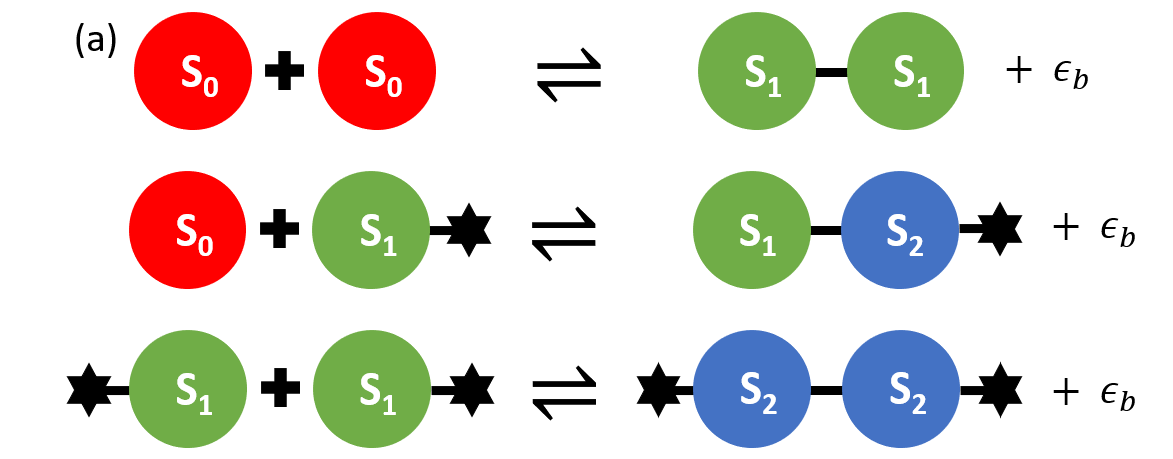
\includegraphics[width=.7\textwidth]{scheme_03.png}
}
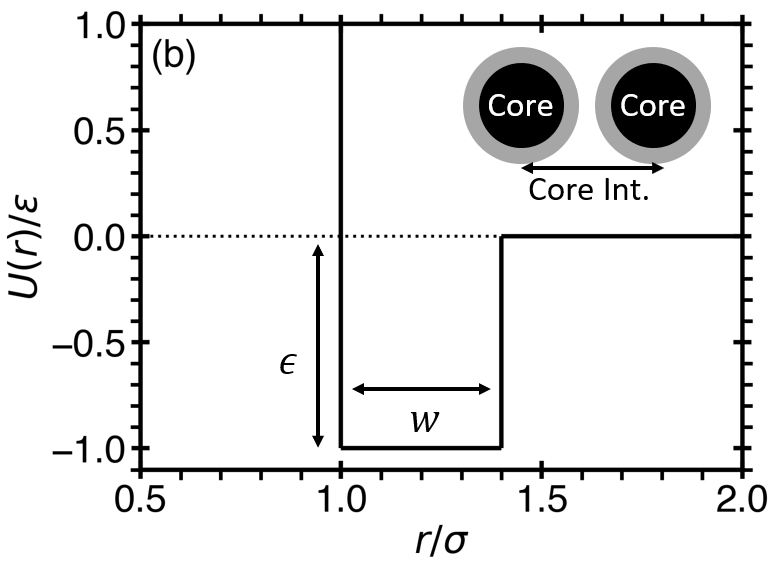
\includegraphics[width=0.32\linewidth]{IntFig1a.png}
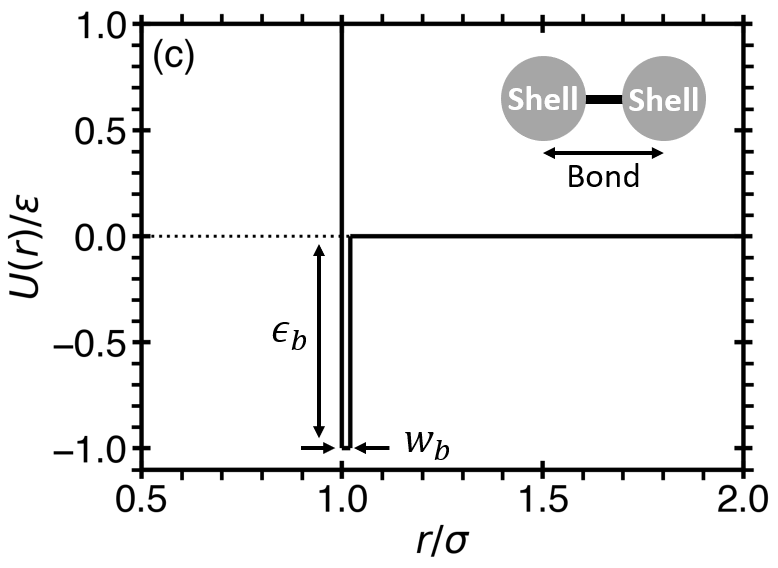
\includegraphics[width=0.32\linewidth]{IntFig1b.png}
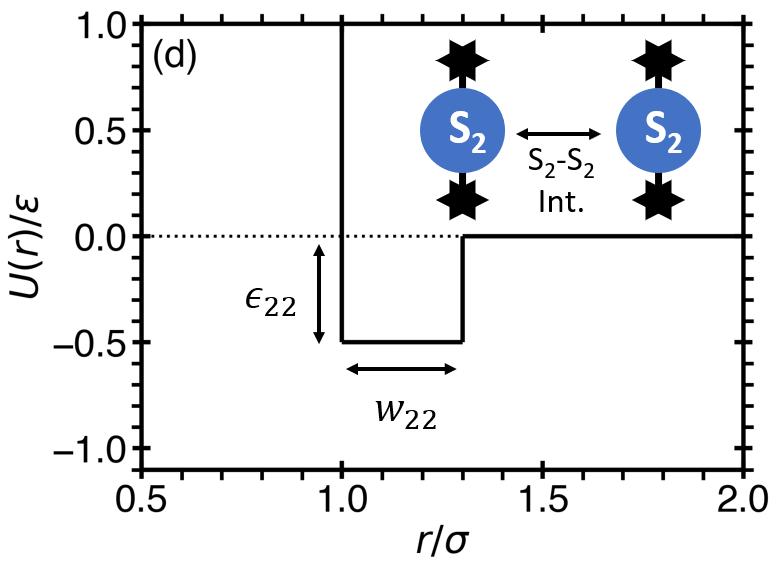
\includegraphics[width=0.32\linewidth]{IntFig1c.png}
\caption{Reactions and interactions in the maximum-valence model. (a) The three types of covalent bond-forming reversible chemical reactions that may occur in the system. If two atoms without bonds (S$_0$) collide with each other, they may form a bond and become S$_1$ atoms. If a S$_0$ and S$_1$ atom collide, they may form a bond and become S$_1$ and S$_2$ atoms, respectively. If two S$_1$ atoms collide with each other, they form an additional bond and become S$_2$ atoms. (b-d) The three major interactions between atoms, in which each atom is composed of a core and shell, both with a radius $\sigma$ and mass $m$. $U(r)$ is the pair potential energy and $r$ is the distance from the center of an atom. (b) The cores of each atom interact with an attractive square well of depth $\epsilon=1$ and width $w=0.4$. (c) The shells may react to form covalent bonds that consist of a narrow well with depth $\epsilon_{b} = 1$ and width $w_{b}=0.02$. (d) Phase segregation is coupled to polymerization via the additional attractive interactions between atoms in state S$_2$, described by a square well of depth $\epsilon_{22} = 0.5$ and width $w_{22}=0.3$.
}
\label{fig1}
\end{figure*}

To verify our hypothesis, we implement these three ingredients of interactions via an event-driven MD technique \cite{Alder1959,Rapaport2004}; in particular, we use a discrete MD package (DMD) that only includes particles interacting through spherically-symmetric step-wise potentials, which may form bonds via reversible reactions \cite{Buldyrev_Application_2008}. We simulate an NVT ensemble of $N=1000$ atoms in a cubic box with periodic boundaries at various constant densities and temperatures. The temperature is controlled by a Berendsen thermostat \cite{Berendsen1984}. The van der Waals and covalent-bonding interactions are implemented by separating each atom into two overlapping hard spheres (a core and a shell), with the same diameter $\sigma$ and mass $m$, see Figs.~\ref{fig1}(b-d). The connection between the core and its shell is represented by an infinite square-well potential of width $d\ll\sigma$. The cores and shells of different atoms do not interact with each other. The core represents the atom without its valence electrons. It interacts with other cores via a wide potential well with depth $\epsilon$ and width $w = 0.4\sigma$ (the parameters are chosen as an example, Fig.~\ref{fig1}b), which models the van der Waals interactions in the system. Meanwhile, the shell represents the outer valence electron cloud. It interacts with other shells via a narrow potential well with depth $\epsilon_b = \epsilon$ and width $w_b=0.02\sigma$ (Fig.~\ref{fig1}c), which models the breaking and forming of covalent bonds. In the absence of the shell, this system has a liquid-gas critical point (LGCP) at $\rho_\text{c}^\text{LG}=N/V=0.35\pm0.05$, $T_\text{c}^\text{LG}=1.04\pm0.01$, and $P_\text{c}^\text{LG}=0.094\pm0.005$ \cite{Skibinsky2004}, well above the equilibrium crystallization line, which we force to be at low temperature by selecting the appropriate width, $w$, of the potential. We note that all physical parameters are normalized by the appropriate combination of mass $m$, length $\sigma$, and energy $\epsilon$ units, as used in Ref. \cite{Skibinsky2004}. When the shell interactions are included and the system may form covalent bonds, the location of the LGCP changes, but not significantly. In addition to the wide and narrow wells, we introduce an additional attractive potential well (with depth $\epsilon_{22}=0.5\epsilon$ and width $w_{22}=0.3\sigma$, Fig.~\ref{fig1}d) for the van der Waals interaction between the shells of the atoms with two bonds (both in the state S$_2$), which are not chemically bonded to each other.

In the DMD approach \cite{Buldyrev_Application_2008}, the particles move along straight lines until they collide with other particles, an event which happens when the distance between two particles intercepts the discontinuity of their pair potential, $U(r)$. After the collision, the new velocities are computed using the conservation of total energy and linear and angular momenta of the colliding pair. We note that during either the formation or breaking of a bond, the new state of the reacting particles may modify the potential energy of the interactions with their non-bonded neighboring particles. In our model, this occurs when particles in the state S$_1$ convert to the state S$_2$ (or vice versa). To maintain the conservation of energy, we calculate the change of the total potential energy, $\Delta U$, due to the change of the state of the reacting particles and subtract it from the kinetic energy of the reacting pair. As a consequence, the equations for computing the new velocities \cite{Buldyrev_Application_2008} may not have real solutions. In this case, the bond will not form or break, and the reacting particles will conserve their states through an elastic collision.

\begin{figure}[t]
\centering
{
%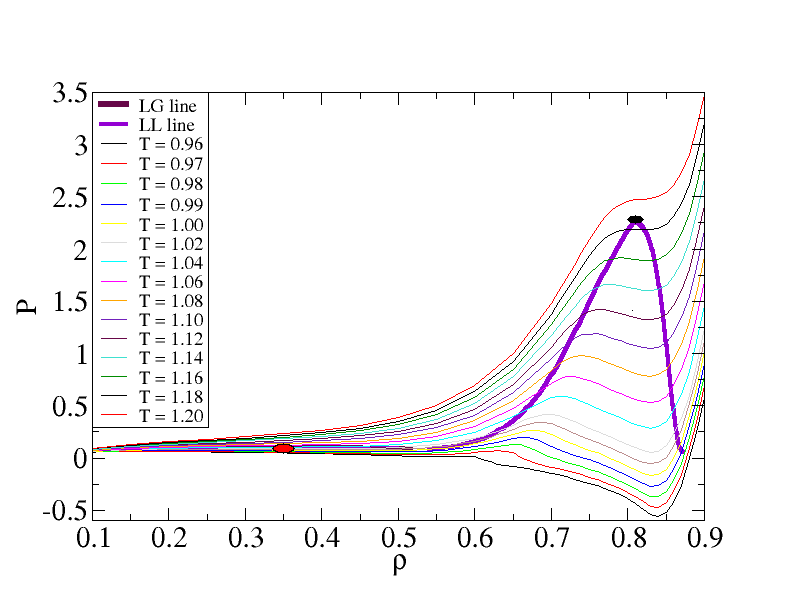
\includegraphics[width=.49\textwidth]{P-rho-full.png}
%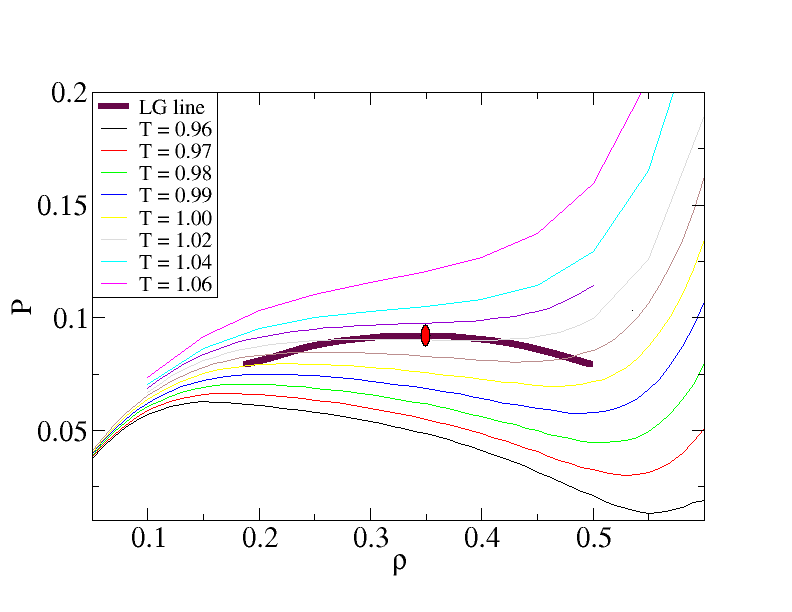
\includegraphics[width=.49\textwidth]{P-rho-inset.png}
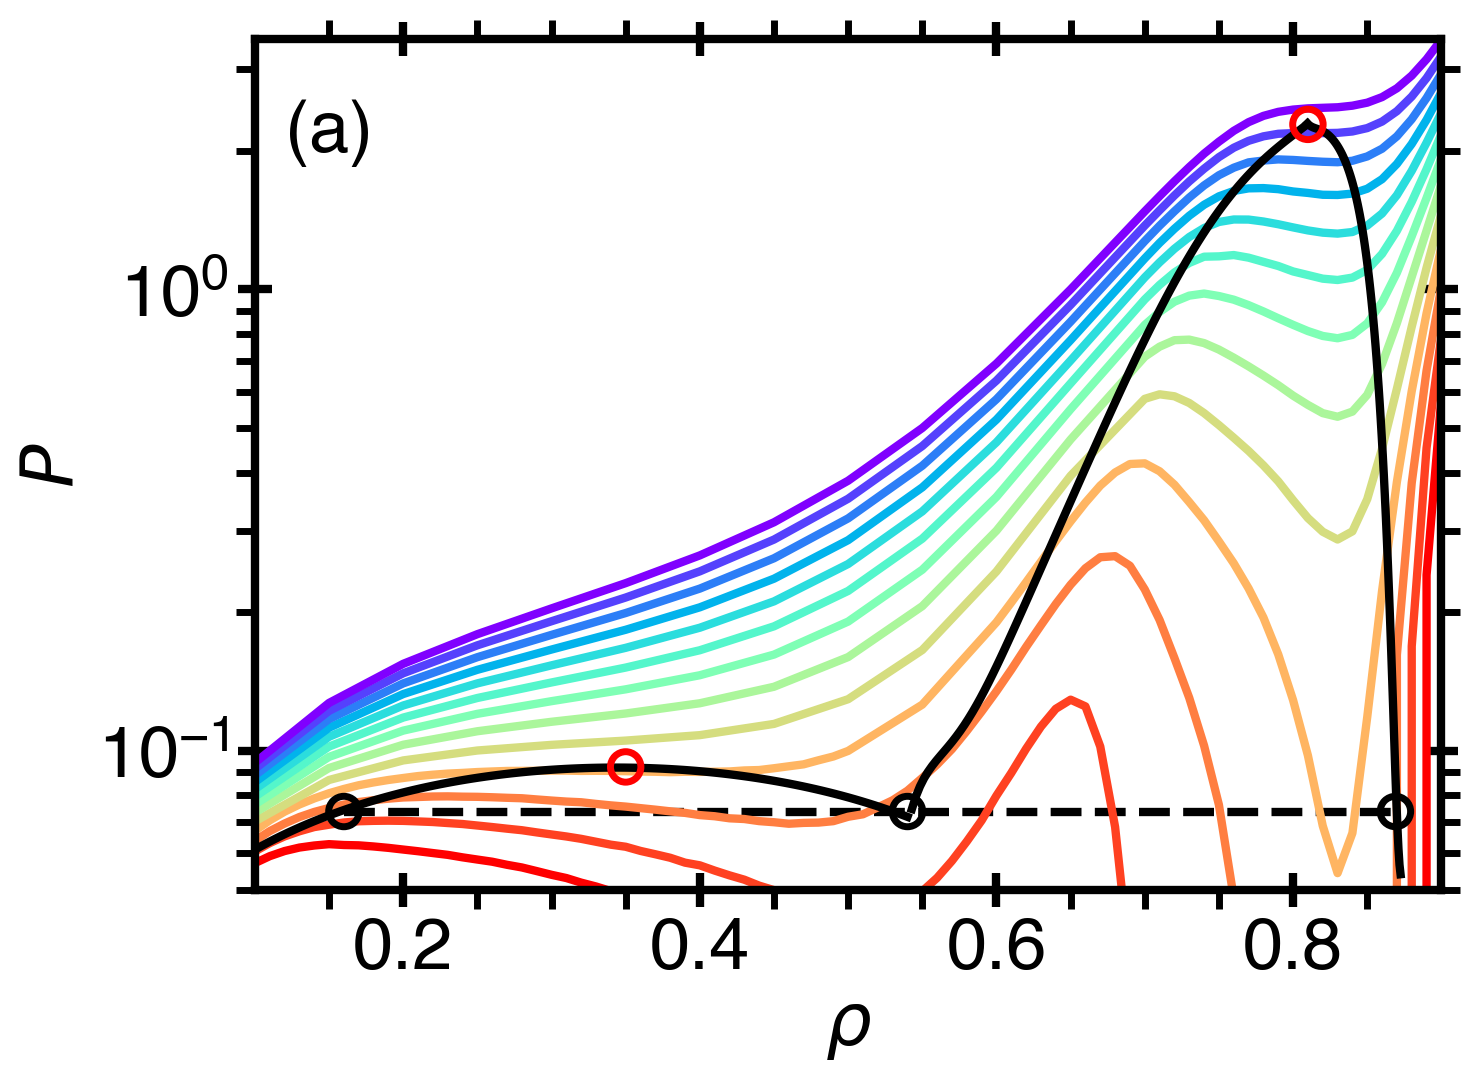
\includegraphics[width=0.9\linewidth]{Fig2a_PrhoDia.png}
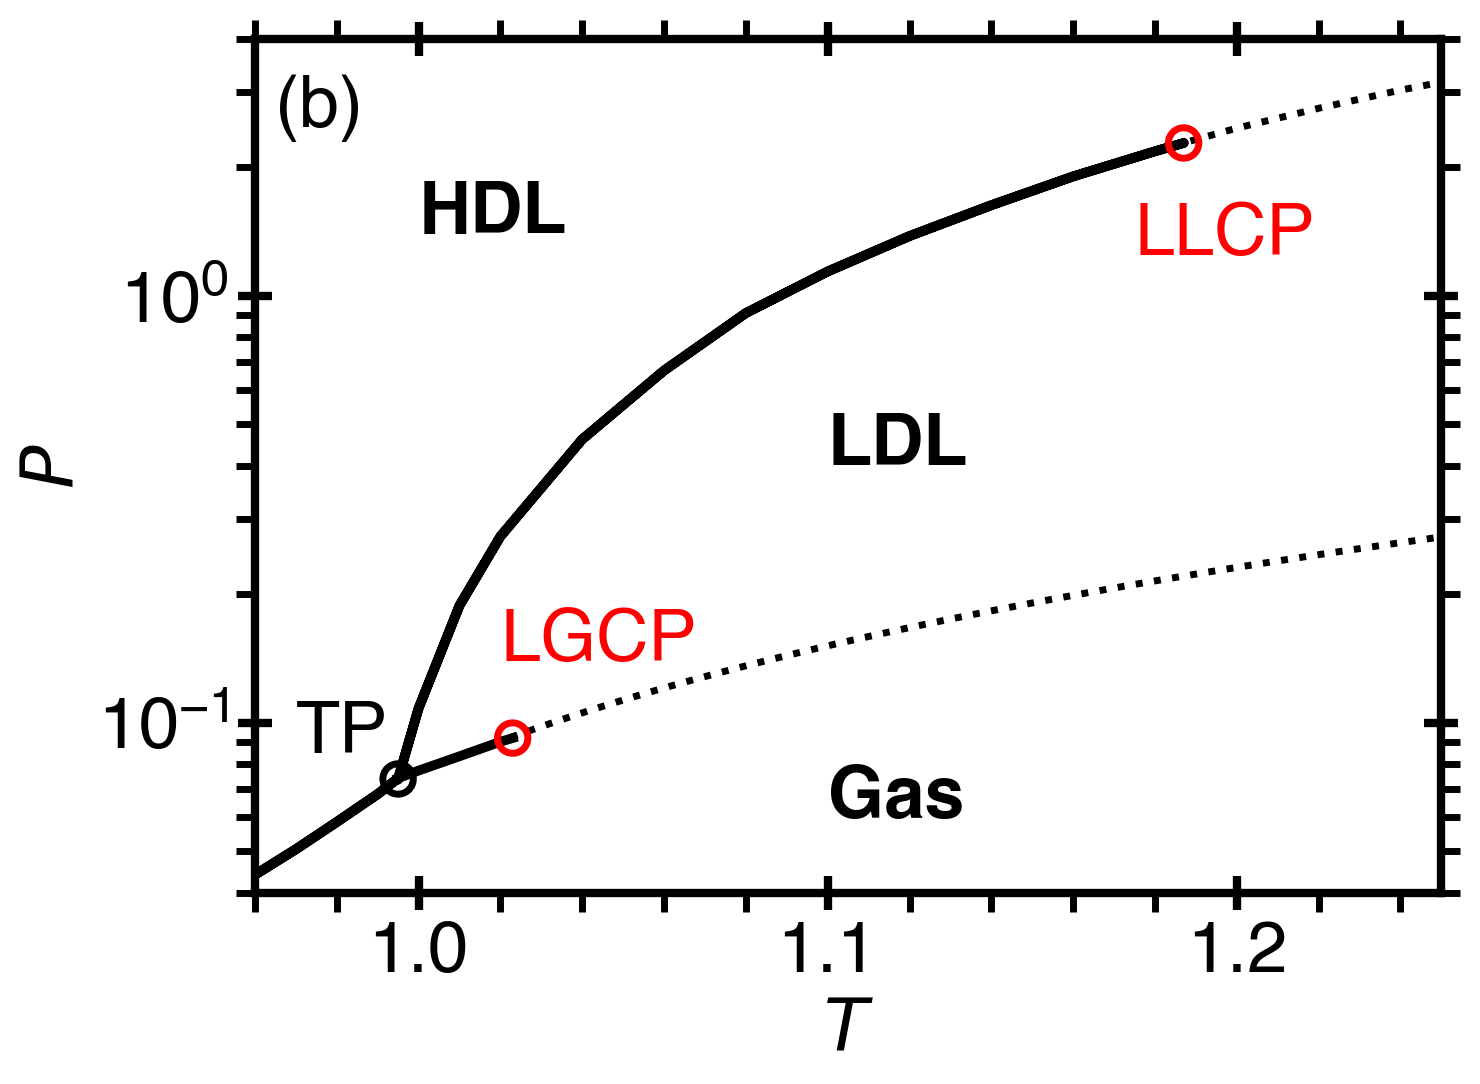
\includegraphics[width=0.9\linewidth]{Fig2b_PTdia.png}
}
\caption{Phase diagrams for the maximum-valence model (with $\epsilon_{22}=0.5$ and $\epsilon_b=1.0$) obtained in an NVT ensemble after $t=10^6$ time units. (a) The isotherms in the $P$-$\rho$ plane are $T=0.96-1.20$ (red-purple) in steps $\Delta T=0.02$. (b) The liquid-gas and liquid-liquid critical isochores in the $P$-$T$ plane are $\rho_\text{c}^\text{LG}=0.35$ and $\rho_\text{c}^\text{LL} = 0.81$ as indicated by the upper and lower dashed lines, respectively. In both figures, the liquid-gas and liquid-liquid coexistence curves are calculated via the Maxwell construction and indicated by the solid curves. The liquid-gas ($T_\text{c}^\text{LG}=1.023$, $P_\text{c}^\text{LG}=0.0922$, $\rho_\text{c}^\text{LG}=0.35$) and liquid-liquid ($T_\text{c}^\text{LL}=1.187$, $P_\text{c}^\text{LL}=2.28$, $\rho_\text{c}^\text{LL}=0.81$) critical points are indicated by the red open circles, while the triple point ($P^\text{TP}=0.0738$, $T^\text{TP}=0.995$) is indicated by the black open circles.}
\label{fig2}
\end{figure}

In this work, we obtain a detailed phase diagram of the model using the values of the square-well depths and widths illustrated in Figs.~\ref{fig1}(b-d). We show that due to the additional attractions between atoms in the state S$_2$ (which are always part of polymer chains), polymerization becomes coupled with phase segregation into two liquid phases with different density: a LDL phase with a smaller fraction of polymerized atoms S$_2$ and a HDL phase with a higher fraction of polymerized atoms. In addition, we investigate the effect of $\epsilon_b$ and $\epsilon_{22}$ on the position of the liquid-liquid (LLCP) and liquid-gas (LGCP) critical points. 

\section*{Results: Liquid-Liquid Phase Transition}
Figure~\ref{fig2}a illustrates isotherms on a pressure-density ($P$-$\rho$) plane, which exhibit two sets of van der Waals loops. The loops correspond to the LGCP, located at low density and pressure, and the LLCP, located at a higher density and pressure. Fig.~\ref{fig2}b illustrates the LG and LL coexistence on a $P$-$T$ plane along with the critical isochores. At the triple point (TP), the gaseous, LDL, and HDL phases coexist. In contrast to the ST2 model for water \cite{Poole1992}, but in agreement with spherically symmetric models \cite{Franzese2001,Luo2015}, the  $P$-$T$ line of the LL coexistence has a positive slope. Simulation snapshots depicted in Fig.~\ref{fig6} show the segregation of polymer-rich, HDL, and polymer-poor, LDL, phases. 

\begin{figure}[t]
	\centering
{
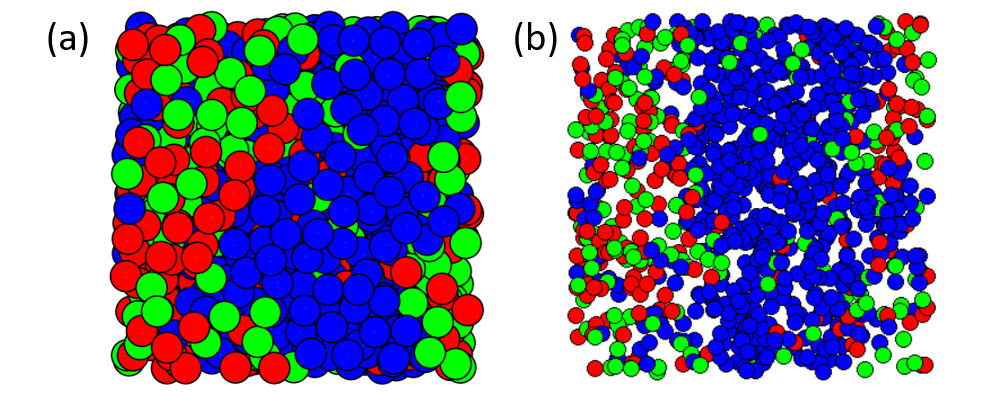
\includegraphics[width=\linewidth]{Particle_SnapShot.png}
%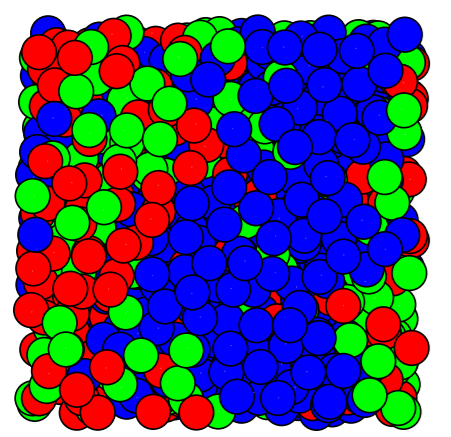
\includegraphics[width=0.19\textwidth]{BS-0.75.png}
%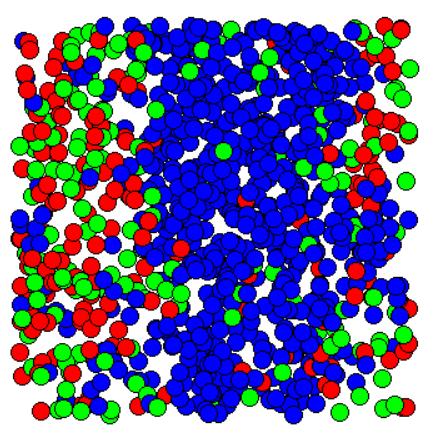
\includegraphics[width=0.19\textwidth]{BS_02.png}
}
\caption{Simulation snapshots of the system exhibiting phase segregation at $T=1.00$ and $\rho=0.75$ in the LL coexistence region for a) $N = 1000$ and b) $N = 8000$ (in which the image size is reduced by a factor of two). Red, green, and blue spheres indicate atom states: S$_0$, S$_1$ and  S$_2$, respectively.}
\label{fig6}
\end{figure}

Figure~\ref{fig3}a presents the LG and LL coexistence curves on a $T$-$\rho$ phase diagram. Although there is a distribution of polymer chains with varying lengths, a simple way to characterize the degree of polymerization is to find the fractions $\phi_0$, $\phi_1$ and $\phi_2$ of atoms in states S$_0$, S$_1$ and S$_2$. Due to the conservation of the number of atoms, $\phi_0+\phi_1+\phi_2 = 1$. The fraction $\phi_2$ was computed based on the asymmetric LL coexistence curve (Fig.~\ref{fig3}a). Remarkably, $\phi_2$ was found to be symmetric and centered around $\phi_2=0.5$ as shown in Fig.~\ref{fig3}b. Consequently, the sum $\phi_0 + \phi_1 = 1-\phi_2$ has the same symmetry. This feature suggests that $\phi_2$ may be viewed as the appropriate order parameter for the LLPT coupled with polymerization. In contrast, the density, $\rho -\rho_\text{c}^\text{LG}$, is the order parameter for the LGPT as commonly accepted. The symmetric nature of $\phi_2$, and the fact that S$_1$ atoms are the intermediate states in the formation of polymer chains, enables a two-state thermodynamic approach \cite{Anisimov2018} by reducing this model to two alternative states, with fractions $\phi_2$ and $\phi_0$ + $\phi_1$. This approach would generate the complete Gibbs energy for the system, such that one would be able to predict thermodynamic properties (\textit{e.g.}, isothermal compressibility, volumetric expansivity, and heat capacity). 

The LLPT coexistence curve on the $T$-$\langle n\rangle$ plane (Fig.~\ref{fig3}c), where $\langle n\rangle$ is the average length of a polymer chain among those containing at least one atom in state S$_2$, namely trimers or longer polymer chains. The strong temperature dependence of $\langle n\rangle$ in the phase segregation region proves that the LLPT is associated with polymerization. Neither $\phi_2$ nor $\langle n\rangle$ shows any discontinuity as a function of density and temperature, although $\langle n\rangle$ shows a strong asymmetry toward the HDL phase. 

%In addition, we observed that the life time of the covalent bonds for $T>1$ is very small, such that the polymer chains frequently break, and the diffusion in both phases is fast and the model easily equilibrates. This is in the unique difference between phase transitions in this model and in models of water, where the diffusivity of the LDL phase is orders of magnitude smaller than of the HDL phase \cite{Xu2005}, such that the LLPT is submerged below the equilibrium crystallization line \cite{Gallo2016}.

\begin{figure*}[t]
\centering
{
%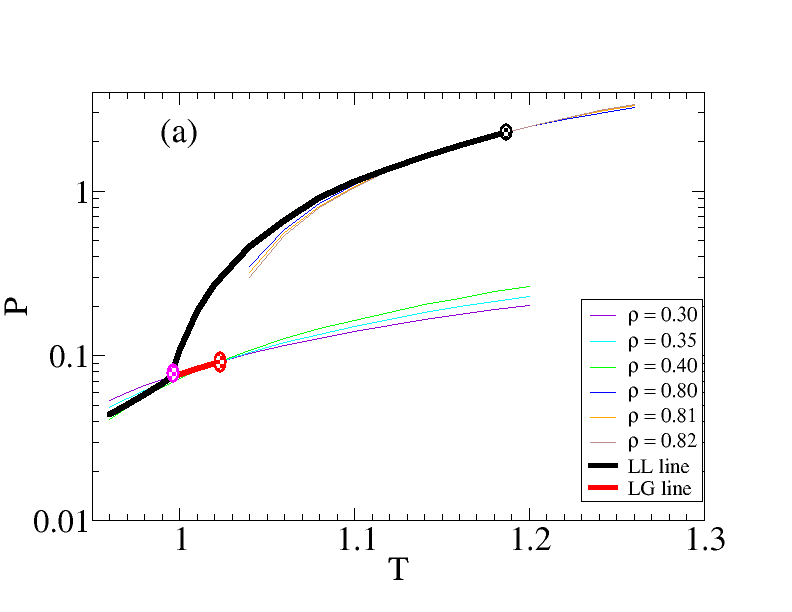
\includegraphics[width=.49\textwidth]{P-T-full.png}
%\includegraphics[width=.49\textwidth]{binodal-full.png}
%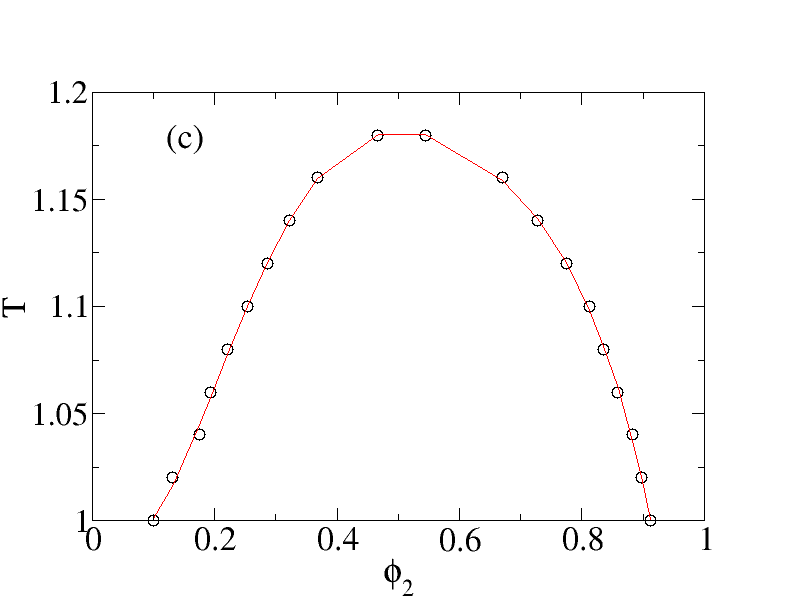
\includegraphics[width=.49\textwidth]{binodal-f3.png}
%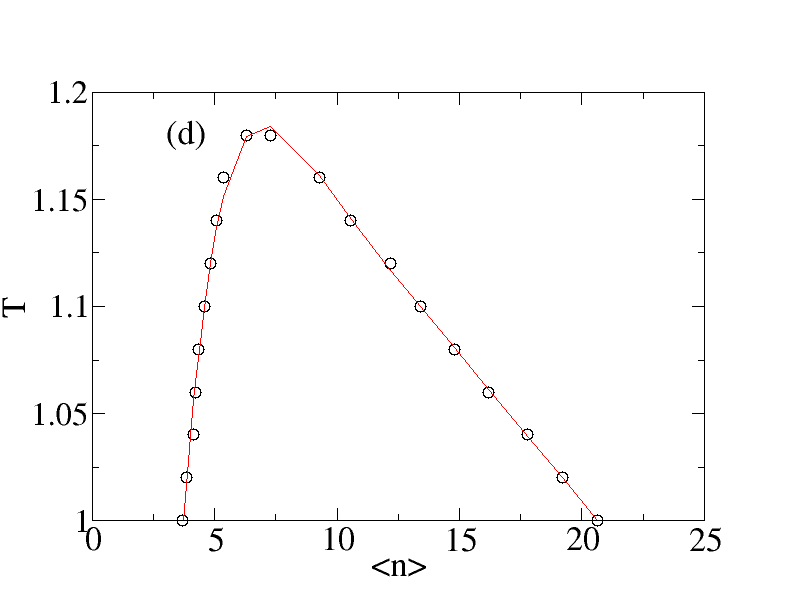
\includegraphics[width=.49\textwidth]{binodal-n1.png}

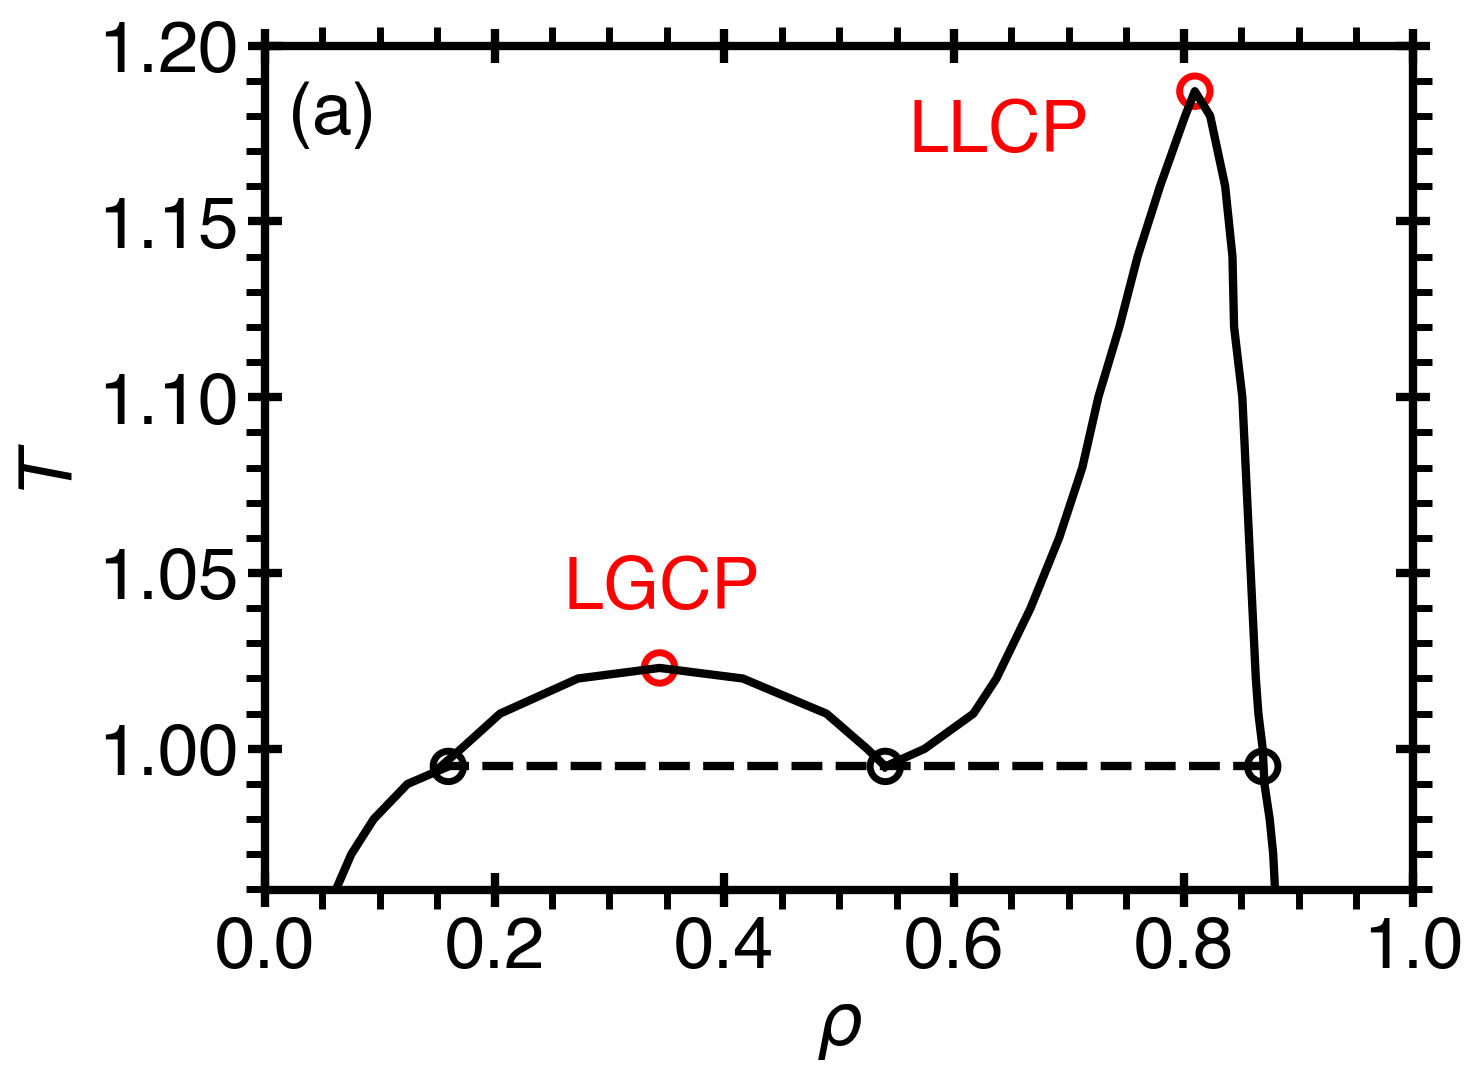
\includegraphics[width=0.32\linewidth]{Fig3a_Trho.png}
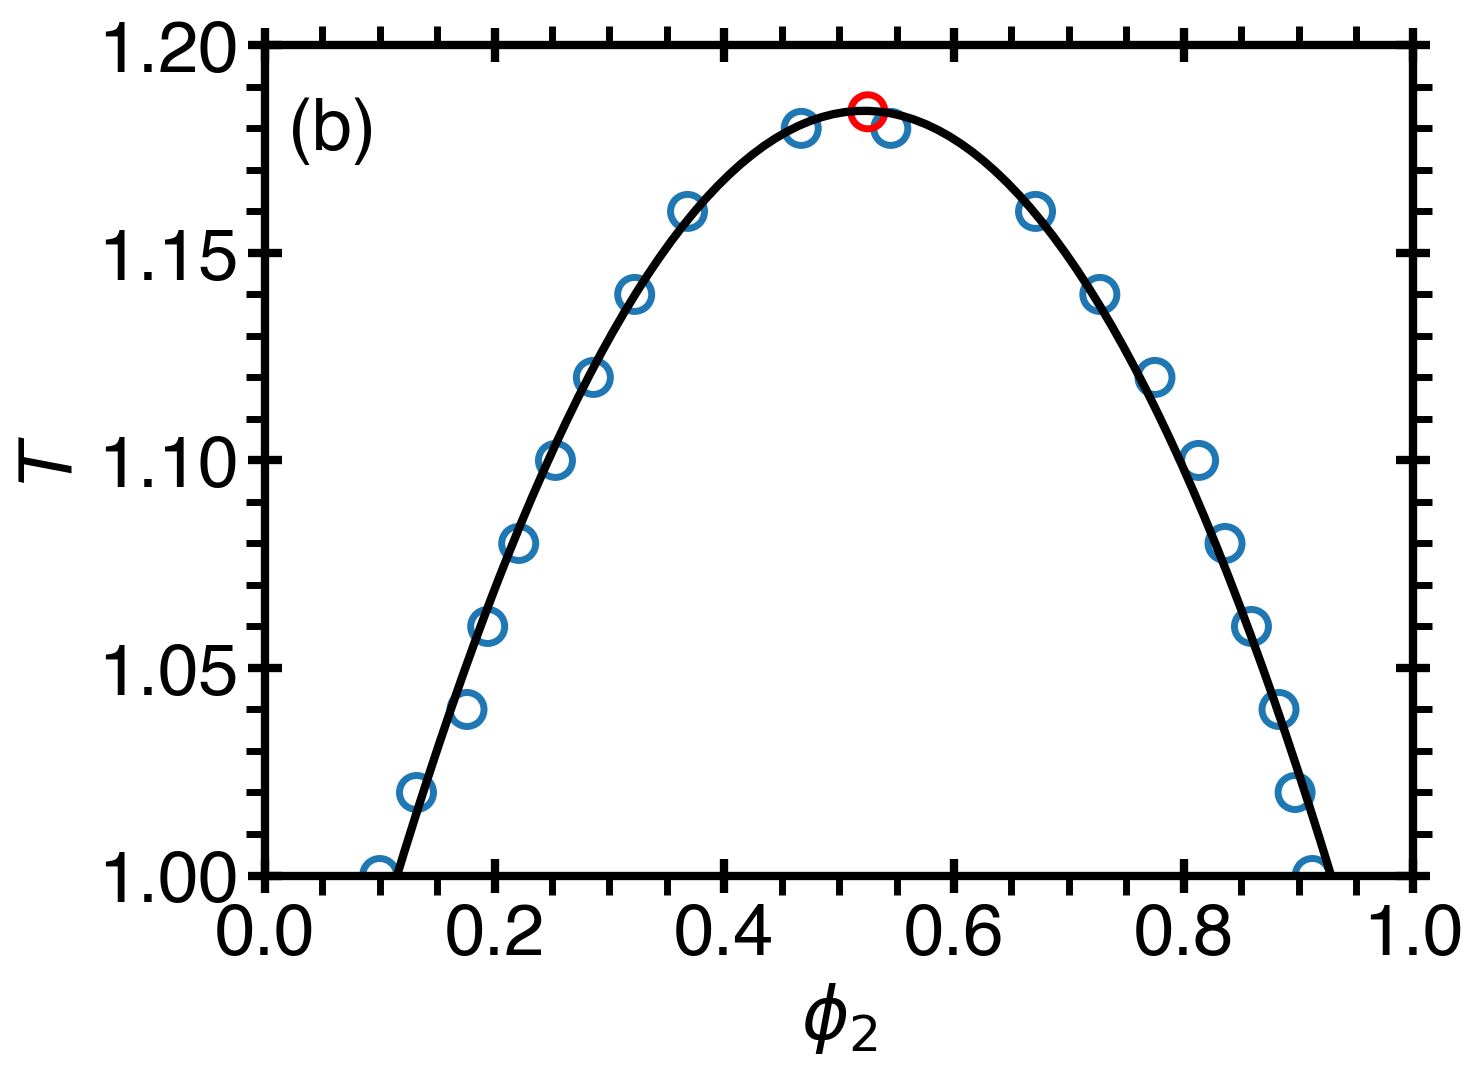
\includegraphics[width=0.32\linewidth]{Fig3b_Tphi2.png}
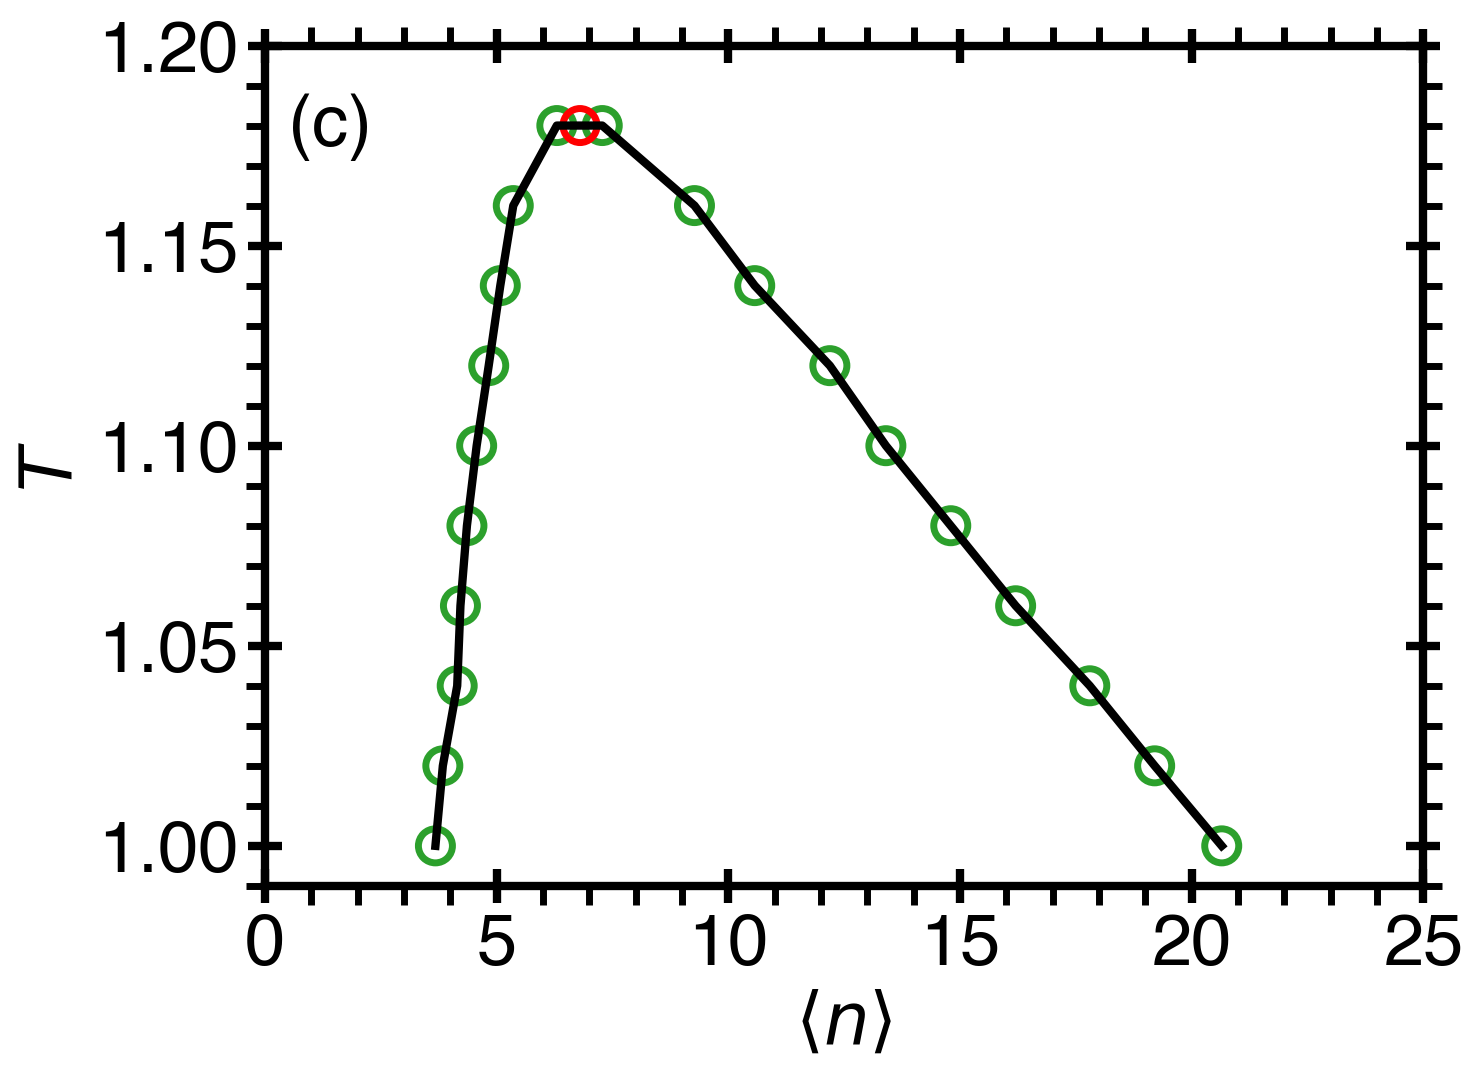
\includegraphics[width=0.32\linewidth]{Fig3c_Tn.png}
}
\caption{(a) $T$-$\rho$ phase diagram for the maximum-valence model (with $\epsilon_{22}=0.5$ and $\epsilon_b=1.0$) obtained in an NVT ensemble after $t=10^6$ time units. The temperature dependence of the fraction of atoms with two bonds, $\phi_2$, (b) and the average chain-length, $\langle n\rangle$, (c) in two coexisting liquid phases. The simulation data in (b) is fit to a second order polynomial, while in (c) the curve is provided as a guide.}
\label{fig3}
\end{figure*}


To illustrate the structural differences between the LDL and HDL phases, we show the density correlation function, $g(r)$, and the structure factor, $S(q)$, for several densities at constant temperature near the LL coexistence computed for the atom cores (Fig.~\ref{fig5}). The $g(r)$ shows a sharp peak corresponding to the covalent bond length $r=1.02\sigma$, in  the HDL phase. Correspondingly, the structure factor shows a shift in the first peak to a larger wavenumber $q$, while the second peak changes due to polymerization. This change is similar to what was observed in a recent experiment on sulfur \cite{Henry2020}. In addition, $S(q)$ shows a dramatic increase as $q\to 0$ for the points corresponding to the equilibrium between two liquid phases (see Fig.~\ref{fig6}), which is indicative of the divergence of the isothermal compressibility.

\begin{figure}[t]
\centering
{
%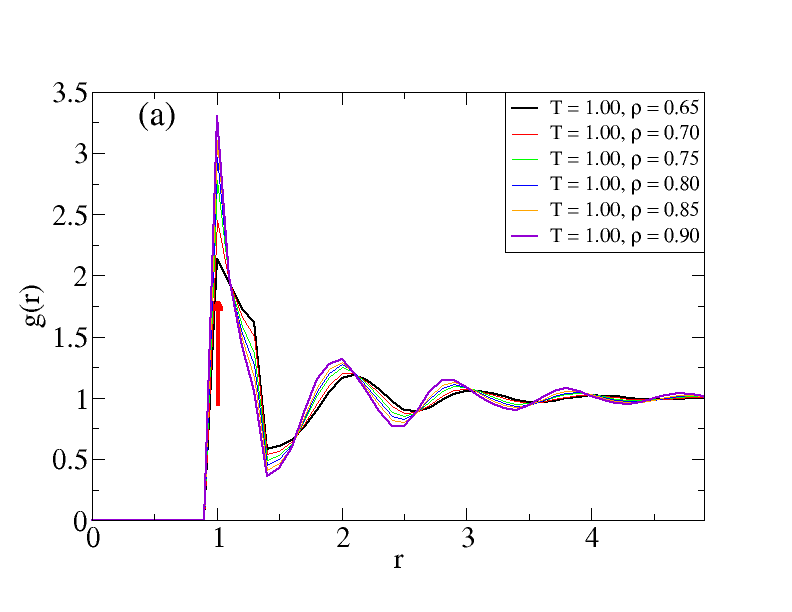
\includegraphics[width=.46\textwidth]{gr-all.png}
%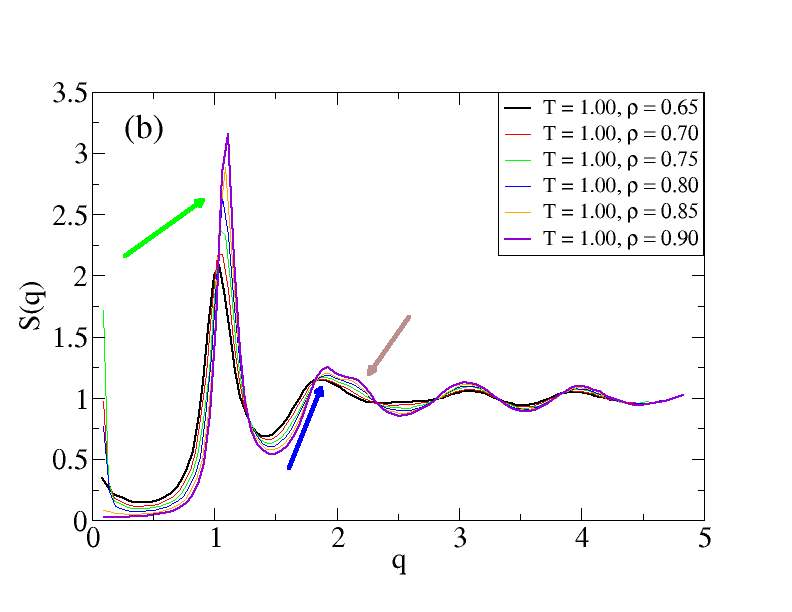
\includegraphics[width=.46\textwidth]{sq-all.png}
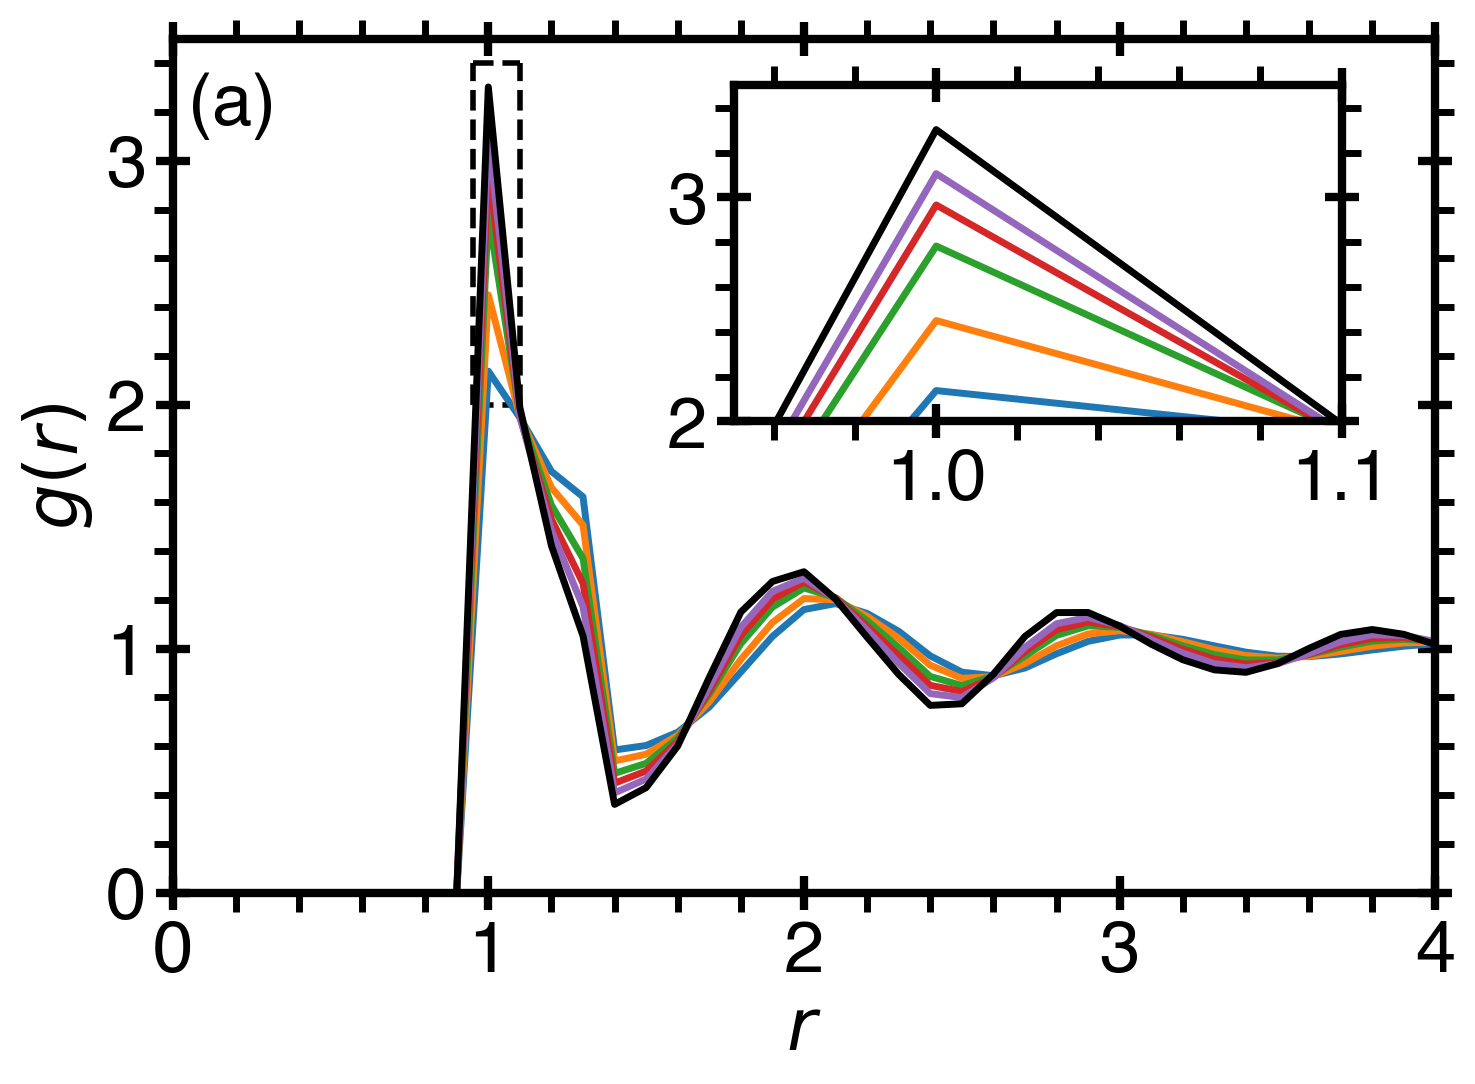
\includegraphics[width=.9\linewidth]{Fig4a_gr.png}
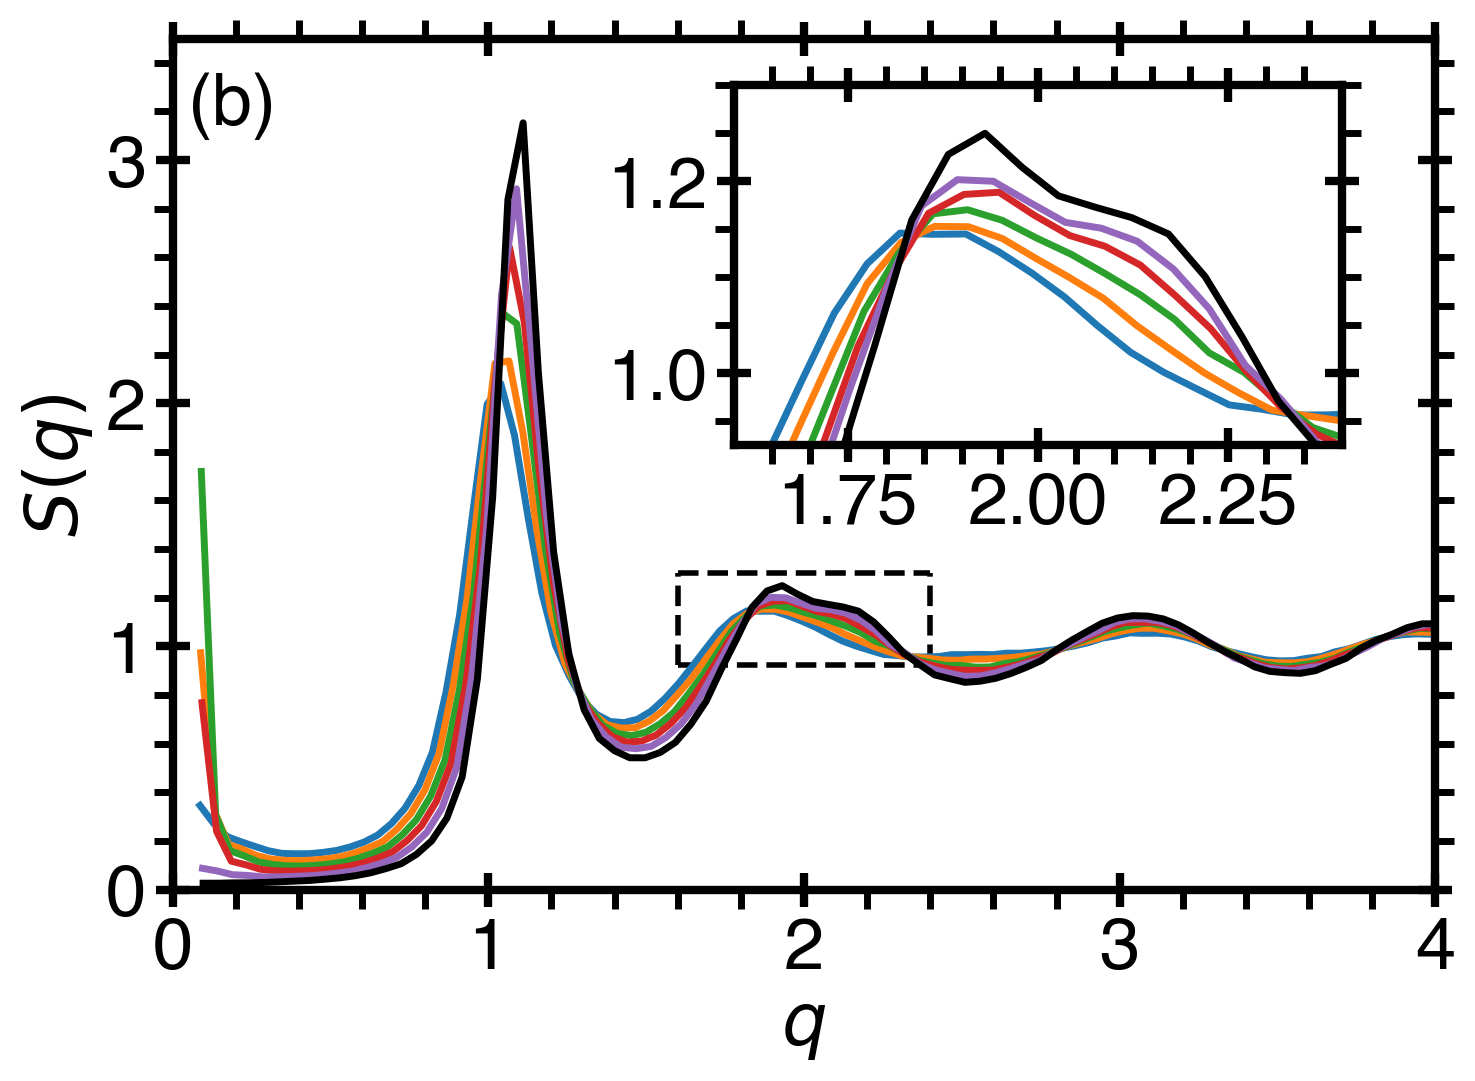
\includegraphics[width=.9\linewidth]{Fig4b_sq.png}
}
\caption{(a) The density correlation function $g(r)$ and (b) the structure factor $S(q)$ across the liquid-liquid transition at $T=1.00$ for densities of $\rho=0.65$ (blue), $\rho=0.70$ (orange), $\rho=0.75$ (green), $\rho=0.8$ (red), $\rho=0.85$ (purple), and $\rho=0.90$ (black). In (a), the sharp peak, around $r=1$ (in units of $\sigma$), corresponds to the length of the covalent bond, which increases upon increasing density. Simultaneously, in (b), the maximum of the structure factor (the first peak) shifts to larger wavenumbers upon increasing density, while the second peak acquires a characteristic bump, similar to what was recently observed in sulfur \cite{Henry2020}. The divergence of the structure factor at $q=0$ indicates the divergence of the isothermal compressibility in the vicinity of the LLCP. The insets (dashed boxes) highlight the behavior of the maximum of the correlation function and second peak of the structure factor.}
\label{fig5}
\end{figure}

\section*{Critical Points: Comparison with Sulfur}
For the values of parameters considered in the previous sections, the system acquires a LLPT terminating at a second critical point, located at $T_\text{c}^\text{LL}=1.187$, $P_\text{c}^\text{LL}=2.28$ and $\rho_\text{c}^\text{LL}=0.81$. We note that the pressure and density for the LLCP are much larger than for the LGCP, while their temperatures are comparable. A qualitatively similar relationship between the critical points exists in real sulfur. In sulfur, the LGCP is located at $T_\text{c}^\text{LG}=\SI{1314}{\kelvin}$, $P_\text{c}^\text{LG}=\SI{20.7}{\mega\pascal}$, and $\rho_\text{c}^\text{LG}=\SI{563}{\kilogram/\meter^3}$ \cite{Lide2003}, while the LLCP is located at $T_\text{c}^\text{LL}=\SI{1035}{\kelvin}$, $P_\text{c}^\text{LL}=\SI{2.15}{\giga\pascal}$, and $\rho_\text{c}^\text{LL}\approx \SI{2000}{\kilogram/\meter^3}$ \cite{Henry2020}.
To compare the maximum-valence model with sulfur, we consider the ratios of the critical parameters for the model: \red{$P_r = P_\text{c}^\text{LL}/P_\text{c}^\text{LG}=25$, $\rho_r= \rho_\text{c}^\text{LL}/\rho_\text{c}^\text{LG}=2.4$, and $T_r = T_\text{c}^\text{LL}/T_\text{c}^\text{LG}=1.16$, with the ratios for sulfur:  $P_r^{S} = P_\text{c}^\text{LL}/P_\text{c}^\text{LG}=104$, $\rho_r^S=\rho_\text{c}^\text{LL}/\rho_\text{c}^\text{LG}=3.4$, and $T_r^{S} =T_\text{c}^\text{LL}/T_\text{c}^\text{LG}=0.78$}. By tuning the interaction parameters of the model, one could better match the simulated critical points and the real ones.

\begin{table}
\caption{Liquid-gas (LGCP) and liquid-liquid (LLCP) critical points for different parameters of the model for $w_a=0.4$}
\centering
\begin{tabular}{ |c||r|r| } 
 \hline
    $w_a=0.4$ & $\epsilon_b=0.5$ & $\epsilon_b=1.0$ \\ 
  \hline
  \hline
 \multirow{3}{4em}{$\epsilon_{22}=0.4$} &  (a) $T_c^\text{LG}=1.00$,  $T_c^\text{LL}=1.00$  &  (b) $T_c^\text{LG}=1.04$, $T_c^\text{LL}=0.94 $ \\
 &     $P_c^\text{LG}=0.09$, $P_c^\text{LL}=3.26$ & $P_c^\text{LG}=0.09$, $P_c^\text{LL}=0.36$ \\
 & $\rho_c^\text{LG}=0.35$, $\rho_c^\text{LL}=0.86$ &  $\rho_c^\text{LG}=0.36$, $\rho_c^\text{LL}=0.76$ \\ 
 \hline
 
  \multirow{3}{4em}{$\epsilon_{22}=0.5$} &  (c) $T_c^\text{LG}=1.02$, $T_c^\text{LL}=1.06$ &  (d) $T_c^\text{LG}=1.02$, $T_c^\text{LL}=1.18$ \\
 &  $P_c^\text{LG}=0.09$, $P_c^\text{LL}=3.34$ & $P_c^\text{LG}=0.09$, $P_c^\text{LL}=2.28$ \\
 & $\rho_c^\text{LG}=0.35$, $\rho_c^\text{LL}=0.87$ & $ \rho_c^\text{LG}=0.34$, $\rho_\text{c}^\text{LL}=0.81$ \\ 
 \hline

\end{tabular}
\label{Table1}
\end{table}

\begin{table}
\caption{Liquid-gas (LGCP) and liquid-liquid (LLCP) critical points for different parameters of the model for $w_a=0.7$}


\centering
\begin{tabular}{ |c||r|r|} 
 \hline
    $w_a=0.7$ & $\epsilon_b=0.00$ & $\epsilon_b=0.50$  \\ 
  \hline
  \hline
 \multirow{3}{4em}{$\epsilon_{22}=0.50$} &   (a) $T_c^\text{LG}=1.59$,  $T_c^\text{LL}=1.24$  &   (b) $T_c^\text{LG}=X$, $T_c^\text{LL}=X$ \\
 &  $P_c^\text{LG}=0.15$, $P_c^\text{LL}=7.64$ & $P_c^\text{LG}=X$, $P_c^\text{LL}=X$  \\
 & $\rho_c^\text{LG}=0.27$, $\rho_c^\text{LL}=0.89$ & $\rho_c^\text{LG}=X$, $\rho_c^\text{LL}=X$ \\
 \hline
 
  \multirow{3}{4em}{$\epsilon_{22}=0.60$} &   (c) $T_c^\text{LG}=1.64$, $T_c^\text{LL}=1.56$ &  (d) $T_c^\text{LG}=1.67$, $T_c^\text{LL}=1.42$  \\ 
  & $P_c^\text{LG}=0.13$, $P_c^\text{LL}=12.0$ & $P_c^\text{LG}=0.12$, $P_c^\text{LL}=2.20$ \\ 
  & $\rho_c^\text{LG}=0.28$, $\rho_c^\text{LL}=0.90$ & $\rho_c^\text{LG}=0.28$, $\rho_\text{c}^\text{LL}=0.85$ \\ 
 \hline 
 

\end{tabular}
\label{Table2}
\end{table}



To understand the effect of the covalent bond strength and the attraction energy of polymeric atoms on the location of the LGCP and LLCP, we determined the critical points for four sets of interaction energies \red{for width, $w=0.4$,} presented in Table~\ref{Table1}. Each of the parameter sets produced a LLCP at much higher pressures than the LGCP, which practically remains the same as for the square-well model without bonds \cite{Skibinsky2004}. We observed that the reduction of the interaction energy from $\epsilon_{22}=0.5$ to $\epsilon_{22}=0.4$ proportionally reduces the liquid-liquid critical temperature from $T_\text{c}^\text{LL}=1.187$ (Table 1d) to $T_\text{c}^\text{LL}=0.94$ (Table 1b), while also significantly reducing the critical pressure from $P_\text{c}^\text{LL}=2.28$ (Table 1d) to $P_\text{c}^\text{LL}=0.36$ (Table 1b). This indicates that the attraction between atoms in state S$_2$ is crucial for the existence of the LLPT, since decreasing the interaction energy further would likely decrease $P_\text{c}^\text{LL}$ to negative pressures and, eventually, to a point below the liquid-gas spinodal, where the LLPT disappears. In contrast, decreasing the bond strength from $\epsilon_b = 1.0$ to $\epsilon_b=0.5$ does not show that the LLPT is going to disappear. Decreasing the bond energy produces a slight increase in the critical temperature and density, while only for strong interaction energies the critical pressure significantly increases, \textit{e.g.} at $\epsilon_{22}=0.5$, $P_\text{c}^\text{LL} = 2.28$ increases to $P_\text{c}^\text{LL} = 3.34$ upon decreasing the bond energy. This indicates that decreasing the strength of polymer bonds is not crucial for the existence of the LLPT. \red{In addition, we found that by increasing the strength of the van der Waals attraction between cores to $w=0.7$, the LLCP to LGCP ratio matches much closer to real sulfur. Parameters for $w=0.7$ are shown in Table~\ref{Table2}, where the best combination of parameters was found to be $w = 0.7$, $\epsilon_b = 0.0$, and $\epsilon_{22}=0.5$ (Table~\ref{Table2}a). With these parameters the ratios are $P_\text{c}^\text{LL}/P_\text{c}^\text{LG}=66$, $\rho_\text{c}^\text{LL}/\rho_\text{c}^\text{LG}=3.31$, and $T_\text{c}^\text{LL}/T_\text{c}^\text{LG}=0.78$. The percent difference between the best parameters for our model and real sulfur are:  $\Delta \hat{T}_r = 0.2\%$, $\Delta \hat{\rho}_r = 2.5\%$, and $\Delta \hat{P}_r = 37\%$, where the percent differences are $\Delta\hat{T} = |T_r - T_r^S|/T_r^S$, $\Delta\hat{\rho} = |\rho_r - \rho_r^S|/\rho_r^S$, and $\Delta\hat{T} = |P_r - P_r^S|/P_r^S$, respectively.} At high densities, long polymer chains would exist due to an entropic effect without any bond energy and even for a negative bond energy. Consequently, even though the ratio of critical pressures in our model is lower than in real sulfur, small adjustments to the parameters could better match the experimental ratio. We note that in our work, we observe a gas-LDL-HDL triple, point, while in the recent experimental work on sulfur \cite{Henry2020}, the solid-LDL-HDL triple point is observed. This result may be reproduced in our model by tuning the width of the van der Waals attractive potential between cores of the atoms, $w$, which promotes or suppresses crystallization. 

\section*{Conclusion}
The LLPT recently observed in sulfur \cite{Henry2020} is induced by polymerization. Our results show that the LLPT predicted by the maximum-valence model qualitatively reproduces the LLPT in sulfur at a high pressure and temperature. In this model, the length of the polymer chains remains finite, and the driving force of the transition is the interconversion between atoms with zero, one, and two covalent bonds. Atoms with two bonds attract each other stronger than atoms with zero and one bond. This generates the HDL phase, formed predominantly by atoms with two bonds, which may segregate from the LDL phase, formed predominantly by atoms with no bonds and single-bonded atoms. The two-state thermodynamics of liquid polyamorphism \cite{Anisimov2018, Caupin2021,Longo2021} could be applied in the future to develop the equation of state, which would determine the anomalies of the physical properties in this system, especially near the critical points. LLPTs may occur at high pressures in other maximum-valence models if the maximum coordination number is greater than two \cite{Smallenburg2014}. For a maximum coordination number of one, the LLPT could be associated with dimerization (similar to what has been observed in high-pressure hydrogen \cite{Simpson_Evidence_2016}), while for a maximum coordination number greater than two, it could be associated with gelation.

The qualitative agreement between our model and real sulfur suggests that in sulfur, at high temperatures and pressures, atoms with two covalent bonds attract each other stronger than other atoms lacking the two covalent bonds. This prediction could be tested in the future with a quantum mechanical approach. In addition, future applications could provide an explanation of LLPTs in other elements prone to catenation, such as phosphorus and solutions of biopolymers. It is known that liquid sulfur exists in the form of octomers at low temperatures, while upon heating, it exhibits a lambda transition into a highly polymerized state, when the octomers break and form very long polymer chains \cite{Sauer_Lambda_1967,Bellissent_Sulfur_1994,Kozhevnikov_Sulfur_2004}. In the future, the maximum-valence model could be elaborated to describe this phenomenon.

\acknow{The authors thank Fr\'ed\'eric Caupin, Pablo G. Debenedetti, Francesco Sciortino, and Eugene I. Shakhnovich for useful discussions. This work is a part of the research collaboration between the University of Maryland, Princeton University, Boston University, and Arizona State University supported by the National Science Foundation. The research at Boston University was supported by NSF Award No. 1856496, while the research at the University of Maryland was supported by NSF award no. 1856479. S.V.B. acknowledges the partial support of this research through Bernard W. Gamson Computational Science Center at Yeshiva College.}


%\matmethods{Please describe your materials and methods here. This can be more than one paragraph, and may contain subsections and equations as required. 

%\subsection*{Subsection for Method}Example text for subsection.}

%\showmatmethods{} % Display the Materials and Methods section


\showacknow{} % Display the acknowledgments section

% Bibliography
\bibliography{pnas-sample}

\section{Supplemental Material}


\begin{table*}[h!]
\caption{Liquid-gas (LGCP) and liquid-liquid (LLCP) critical points for different parameters of the model for $w_a=0.7$}
\centering
\begin{tabular}{ |c||r|r|r| } 
 \hline
    $w_a=0.7$ & $\epsilon_b=0.00$ & $\epsilon_b=0.50$ & $\epsilon_b=1,00$ \\ 
  \hline
  \hline
 \multirow{3}{4em}{$\epsilon_{22}=0.55$} &   $T_c^\text{LG}=1.60$,  $T_c^\text{LL}=1.37$  &   $T_c^\text{LG}=1.62$, $T_c^\text{LL}=1.28$  &   $T_c^\text{LG}=1.66$,  $T_c^\text{LL}=1.21$ \\
 &  $P_c^\text{LG}=0.12$, $P_c^\text{LL}=8.90$ & $P_c^\text{LG}=0.12$, $P_c^\text{LL}=4.39$  & $P_c^\text{LG}=0.13$, $P_c^\text{LL}=1.6$ \\
 & $\rho_c^\text{LG}=0.27$, $\rho_c^\text{LL}=0.91$ &  $\rho_c^\text{LG}=0.27$, $\rho_c^\text{LL}=0.82$ &  $\rho_c^\text{LG}=0.26$, $\rho_c^\text{LL}=0.89$ \\ 
 \hline
 
  \multirow{3}{4em}{$\epsilon_{22}=0.60$} &   $T_c^\text{LG}=1.64$, $T_c^\text{LL}=1.56$ &   $T_c^\text{LG}=1.67$, $T_c^\text{LL}=1.42$  &    $T_c^\text{LG}=1.64$, $T_c^\text{LL}=1.31$ \\ 
  & $P_c^\text{LG}=0.13$, $P_c^\text{LL}=12.0$ & $P_c^\text{LG}=0.12$, $P_c^\text{LL}=2.20$& $P_c^\text{LG}=0.15$, $P_c^\text{LL}=5.89$ \\ 
  & $\rho_c^\text{LG}=0.28$, $\rho_c^\text{LL}=0.90$ & $\rho_c^\text{LG}=0.28$, $\rho_\text{c}^\text{LL}=0.85$& $\rho_c^\text{LG}=0.28$, $\rho_\text{c}^\text{LL}=0.80  $ \\ 
 \hline 
 

\end{tabular}
\label{Table3}
\end{table*}


\begin{table*}[h!]
\caption{Liquid-gas (LGCP) and liquid-liquid (LLCP) critical points for different parameters of the model for $w_a$}
\centering
\begin{tabular}{ |c||r|r|r|r|r|r| } 
 \hline
    $w$ & $w=0.40$ & $w = 0.45$ & $w = 0.50$ & $w = 0.55$ & $w = 0.60$ \\
    
    %& $w_a = 1.65$ & $w_a = 1.70$ & $w_a = 1.75$  \\ 
  \hline
  \hline
 \multirow{3}{4em}{$\epsilon_{22}=0.50$}
 &   $T_c^\text{LG}=1.00$, $T_c^\text{LL}=1.37$  
 &   $T_c^\text{LG}=1.10$, $T_c^\text{LL}=1.31$  
 &   $T_c^\text{LG}=1.20$,  $T_c^\text{LL}=1.27$ 
 &   $T_c^\text{LG}=1.27$,  $T_c^\text{LL}=1.29$
 &   $T_c^\text{LG}=1.37$,  $T_c^\text{LL}=1.23$\\
 %&   $T_c^\text{LG}=1.51$,  $T_c^\text{LL}=1.23$
 %&   $T_c^\text{LG}=1.59$,  $T_c^\text{LL}=1.24$
 %&   $T_c^\text{LG}=1.70$,  $T_c^\text{LL}=1.27$ \\
 &  $P_c^\text{LG}=0.10$, $P_c^\text{LL}=11.72$ 
 & $P_c^\text{LG}=0.11$, $P_c^\text{LL}=4.39$  
 & $P_c^\text{LG}=0.13$, $P_c^\text{LL}=1.6$
 & $P_c^\text{LG}=0.13$, $P_c^\text{LL}=1.6$
 & $P_c^\text{LG}=0.13$, $P_c^\text{LL}=1.6$\\
 %& $P_c^\text{LG}=0.13$, $P_c^\text{LL}=1.6$ 
 %& $P_c^\text{LG}=0.13$, $P_c^\text{LL}=1.6$
 %& $P_c^\text{LG}=0.13$, $P_c^\text{LL}=1.6$
 %& $P_c^\text{LG}=0.13$, $P_c^\text{LL}=1.6$ \\
 & $\rho_c^\text{LG}=0.27$, $\rho_c^\text{LL}=0.91$ &  $\rho_c^\text{LG}=0.27$, $\rho_c^\text{LL}=0.82$ &  $\rho_c^\text{LG}=0.26$, $\rho_c^\text{LL}=0.89$ & $\rho_c^\text{LG}=0.26$, $\rho_c^\text{LL}=0.89$ 
 & $\rho_c^\text{LG}=0.26$, $\rho_c^\text{LL}=0.89$ \\ 
 \hline
\end{tabular}
\label{Table4a}
\end{table*}

\begin{table*}[h!]
\caption{Liquid-gas (LGCP) and liquid-liquid (LLCP) critical points for different parameters of the model for $w$}
\centering
\begin{tabular}{ |c||r|r|r|} 
 \hline
    $w$ %& $w_a=1.40$ & $w_a = 1.45$ & $w_a = 1.50$ & $w_a = 1.55$ & $w_a = 1.60$ \\
    
    & $w = 0.65$ & $w_a = 0.70$ & $w_a = 0.75$  \\ 
  \hline
  \hline
 \multirow{3}{4em}{$\epsilon_{22}=0.50$}
 %   $T_c^\text{LG}=1.00$, $T_c^\text{LL}=1.37$  
 %&   $T_c^\text{LG}=1.10$, $T_c^\text{LL}=1.31$  
 %&   $T_c^\text{LG}=1.20$,  $T_c^\text{LL}=1.27$ 
 %&   $T_c^\text{LG}=1.27$,  $T_c^\text{LL}=1.29$
 %&   $T_c^\text{LG}=1.37$,  $T_c^\text{LL}=1.23$\\
 &   $T_c^\text{LG}=1.51$,  $T_c^\text{LL}=1.23$
 &   $T_c^\text{LG}=1.59$,  $T_c^\text{LL}=1.24$
 &   $T_c^\text{LG}=1.70$,  $T_c^\text{LL}=1.27$ \\
 %&  $P_c^\text{LG}=0.10$, $P_c^\text{LL}=11.72$ 
 %& $P_c^\text{LG}=0.11$, $P_c^\text{LL}=4.39$  
 %& $P_c^\text{LG}=0.13$, $P_c^\text{LL}=1.6$
 %& $P_c^\text{LG}=0.13$, $P_c^\text{LL}=1.6$
 %& $P_c^\text{LG}=0.13$, $P_c^\text{LL}=1.6$\\
 & $P_c^\text{LG}=0.13$, $P_c^\text{LL}=1.6$ 
 & $P_c^\text{LG}=0.13$, $P_c^\text{LL}=1.6$
 & $P_c^\text{LG}=0.13$, $P_c^\text{LL}=1.6$ \\
 %& $P_c^\text{LG}=0.13$, $P_c^\text{LL}=1.6$ 
 & $\rho_c^\text{LG}=0.27$, $\rho_c^\text{LL}=0.91$ &  $\rho_c^\text{LG}=0.27$, $\rho_c^\text{LL}=0.82$ &  
 $\rho_c^\text{LG}=0.26$, $\rho_c^\text{LL}=0.89$\\ 
 \hline
\end{tabular}
\label{Table4a}
\end{table*}


\end{document}
